\documentclass{article}

\usepackage{ctex}
\usepackage[left=1.25in,right=1.25in,top=1in,bottom=1in]{geometry}
\usepackage{amsmath}
\usepackage{amssymb}
\usepackage{graphicx}
\usepackage{listings}
\lstset{language=Matlab}   
\lstset{breaklines}              
\lstset{extendedchars=false}
\usepackage[framed,numbered,autolinebreaks,useliterate]{mcode}

\author{张泽宇}
\date{2022年3月6日}
\title{第二周工作总结}

\begin{document}
	\maketitle
	
	{\centering \rule[15pt]{15cm}{0.1em}}
	
	{\noindent\large\textbf{
	这一周的主要进行的工作包括有:
	\begin{itemize}
		\item 模型闭环的初步思考与构建
		\item 基于Simulink的仿真电路搭建
		\item 对样本集的拓展处理
		\item 基于Matlab的简单卷积神经网络搭建
		\item 初步的训练尝试
	\end{itemize}
	产生的问题主要包括:
	下面报告进展,以及一些疑惑。} }
	
	\section{模型闭环的初步思考与构建}
	
	我从以下几个角度思考了深度学习进行电力故障判断所需要的要素:
	
	\begin{enumerate}
		\item 训练数据来源:采用Simulink搭建电路仿真,观测到的指标可以是数据序列,也可以是示波器上的图像。这里有两种不同的思路分支。
		\begin{itemize}
			\item 如果以数据序列作为训练的数据,可以从时间序列预测的方向进行。但是,这种方式的推广性,我认为不太可行。因为在我的认知里,故障检测应该做到即时性,如果等采集到\textbf{一串足够的}时间数据序列之后在进行,可能不太及时。
			\item 如果以示波器上显示的图像作为神经网络的输出,可以从CNN角度着手,类似于图像分类,不同特征在观测量的波形上必然出现不同的特征,利用CNN学习这种特征,从而判断故障种类。同时,这样的图像识别,在即时性上应该比数据序列强。
		\end{itemize}
	
		因此我认为可以将不同情况下(电路正常运行,某处短路,某处断路等)电路模型仿真的结果用示波器显示,然后导出成图像,对图像进行学习。
		
		\item 训练图像的处理:因为仿真的结果必然是少数,无法实现有意义的网络学习与训练,这一问题被称为小样本训练Few-Shot Learning。我查阅了一些资料\footnote{https://zhuanlan.zhihu.com/p/290011942},发现解决这一问题的主要方向有三个,
		
		\begin{enumerate}
			\item 缩小模型需要搜索的空间
			\item 优化搜索最优模型的过程。这两种方法需要一段时间进行探索,可能是解决的思路,这里仅作记录。
			\item 增多训练数据。可以通过1、数据增强,2、基于弱标记样本或无标记样本得到更多目标class样本,3、基于目标Class的小样本数据训练GAN,直接生成目标class的更多样本等方法实现,同上,采用数据增强的方法比较易于上手。
		\end{enumerate}
	
		针对数据增强,初级的方法是对图片进行旋转、翻转、裁剪、增加噪音等操作。考虑到波形识别的特殊性,显然类似于图像左右翻转,上下翻转的变化是不可行的。我想到的方法是,波形部分区域截取,图片饱和度、对比度、亮度的修改,将原始图像按照RGB三色道分开再重新组合,小幅度的旋转,复制等。总之就是在不改变波形的前提下,对图像做尽可能多的“衍生”。
		
		\item 神经网络的搭建:可以借助Matlab中的深度学习设计器APP先对网络的框架进行构造,然后借助其自动检查功能,检查维度是否匹配等,确认无误后再写具体的代码。
		
		但是在网络的结构上,学生有一定的疑问。因为我之前了解到我们设定CNN的相关参数,比如卷积核的大小、激活函数选取、步幅的大小,甚至学习率这些,都是依据经验。所以在我后来训练的过程中,在参数设定上基本是盲目尝试,但是结果都不是特别好,我不清楚是网络的结构不合适,还是参数的设定不合适。
	\end{enumerate}

	这是我初步认为的需要进行的三个主要步骤。每个步骤我又思考了一下可能存在的拓展,但这周是先尝试按照基本的内容进行。
	
	\section{基于Simulink的仿真电路搭建}
	
	我选取了一个全波整流滤波电路,电路结构比较简单,如下图
	
	\begin{figure}[h]
		\centering
		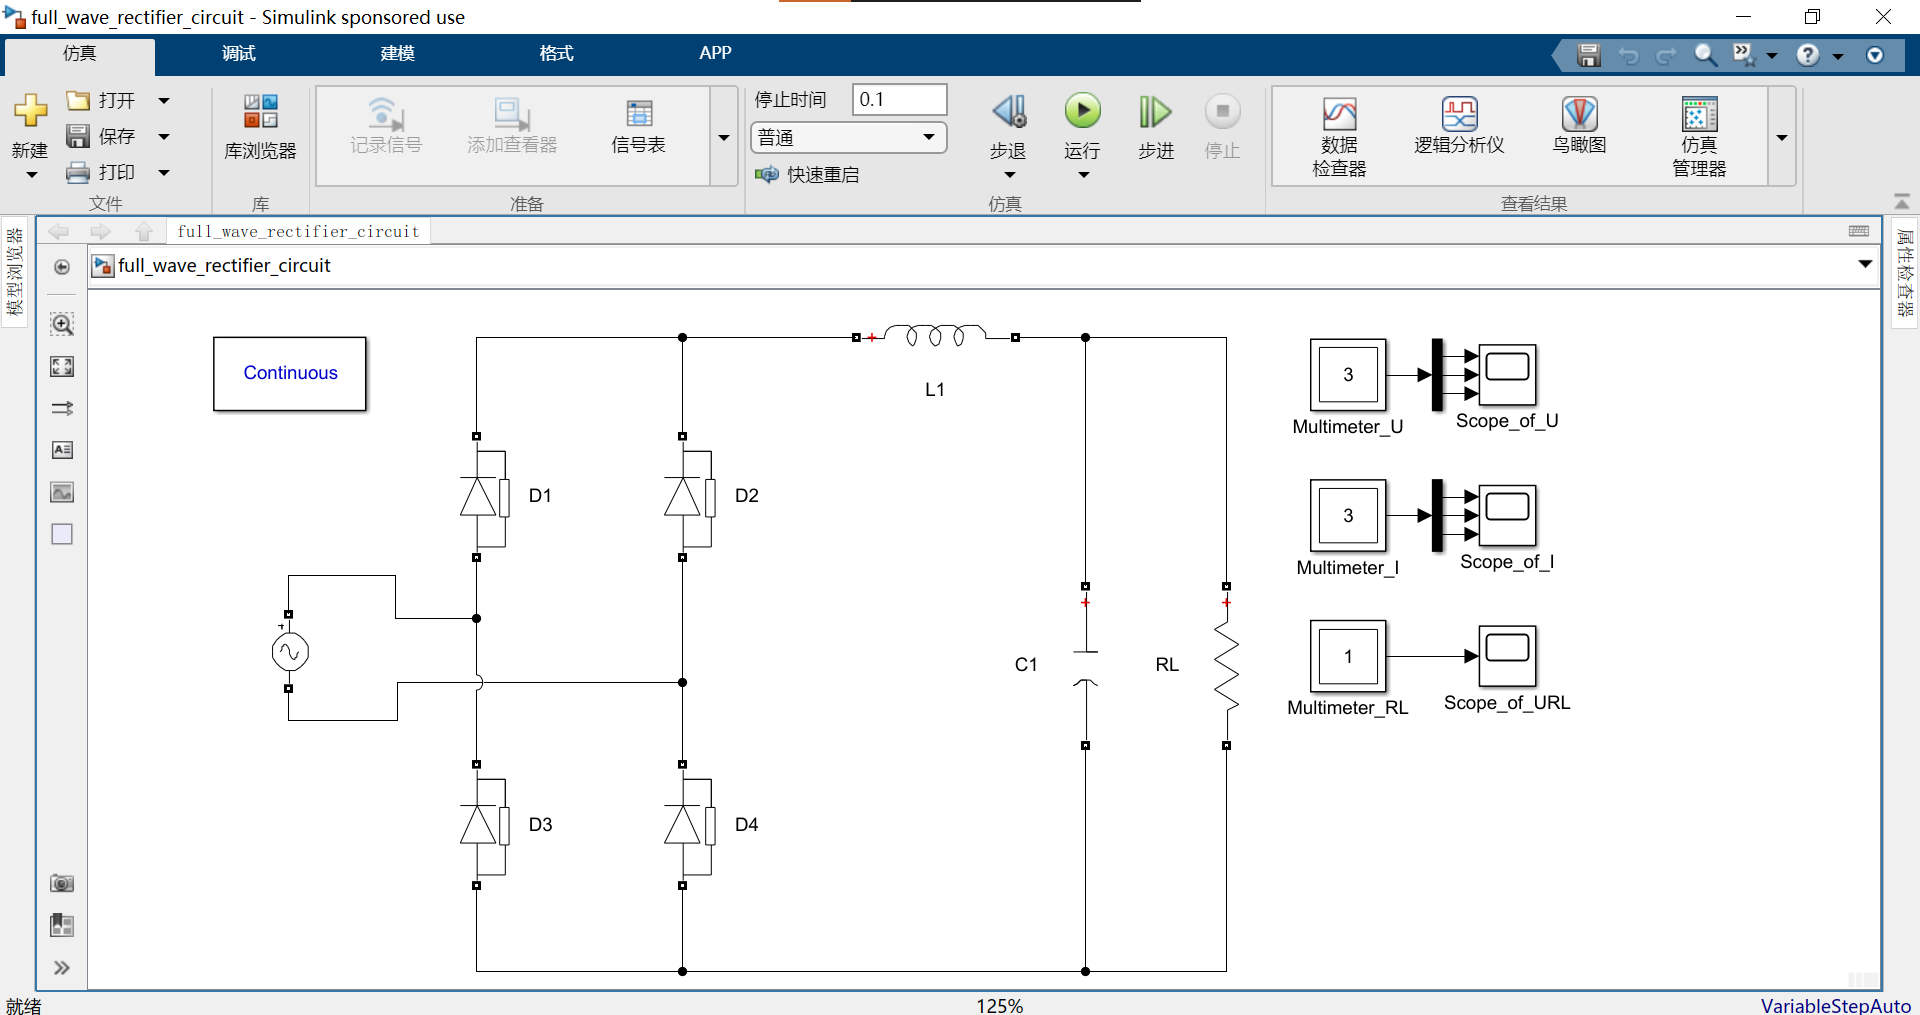
\includegraphics[width=10cm]{figure/full_wave_rectifier.png}
		\caption{全波整流滤波电路}
	\end{figure}
	
	电源只考虑了单相交流电源,然后测量单元用两个万用表分别测量了RLC上的电压电流,最后另用万用表采集训练数据。
	
	正常情况下,RLC上的电压电流如下:
	
	\begin{figure}[h]
		\centering
		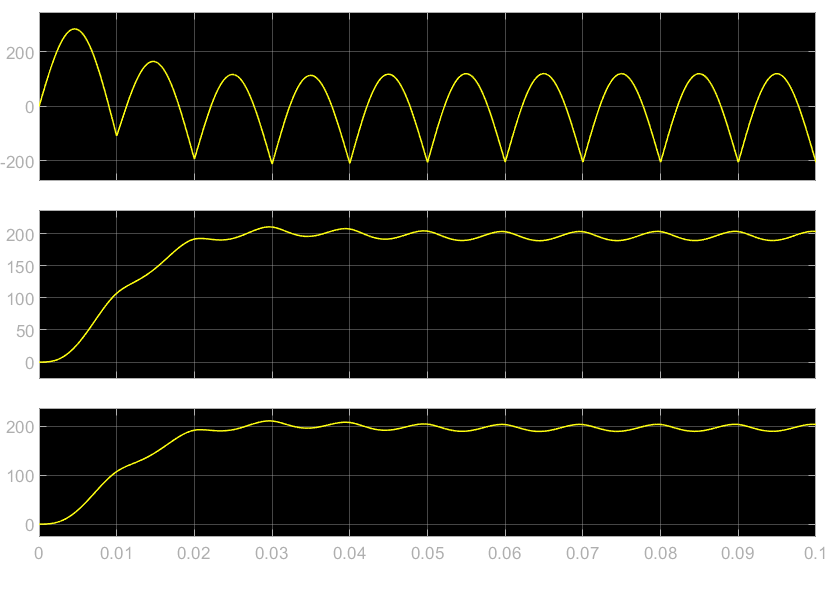
\includegraphics[width=10cm]{figure/normal_U.png}
		\quad
		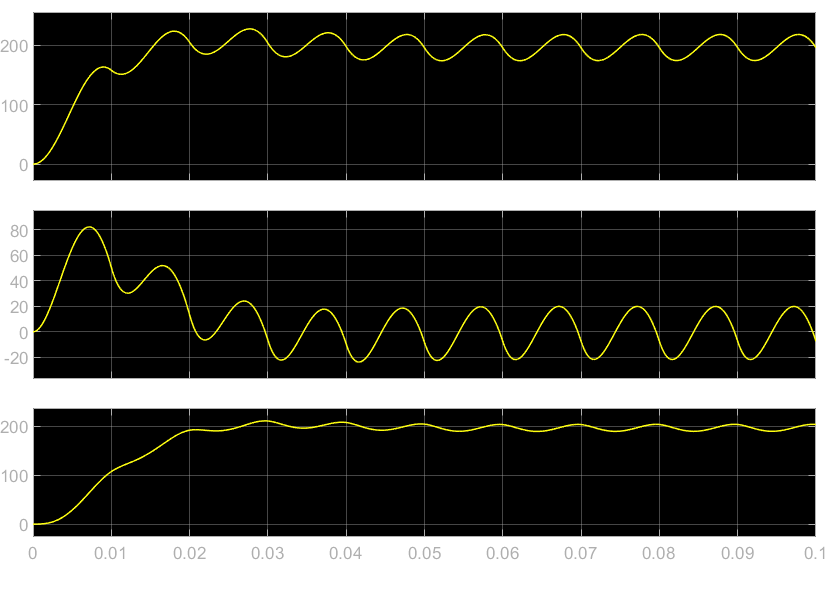
\includegraphics[width=10cm]{figure/normal_I.png}
		\caption{正常情况RLC上的电压电流}
	\end{figure}
	
	之后,用一个breaker模块和step脉冲模块设置支路的开路和短路。我主要设置了四种故障,故障发生在电路仿真开始后0.04s时刻:
	\begin{enumerate}
		\item 二极管D2短路
		\item 二极管D2开路
		\item 二极管D4开路
		\item 电感L开路
	\end{enumerate}
	
	仿真电路以及负载$R_{L}$上的电压如下:
	
	\begin{figure}[bhtp]
		\centering
		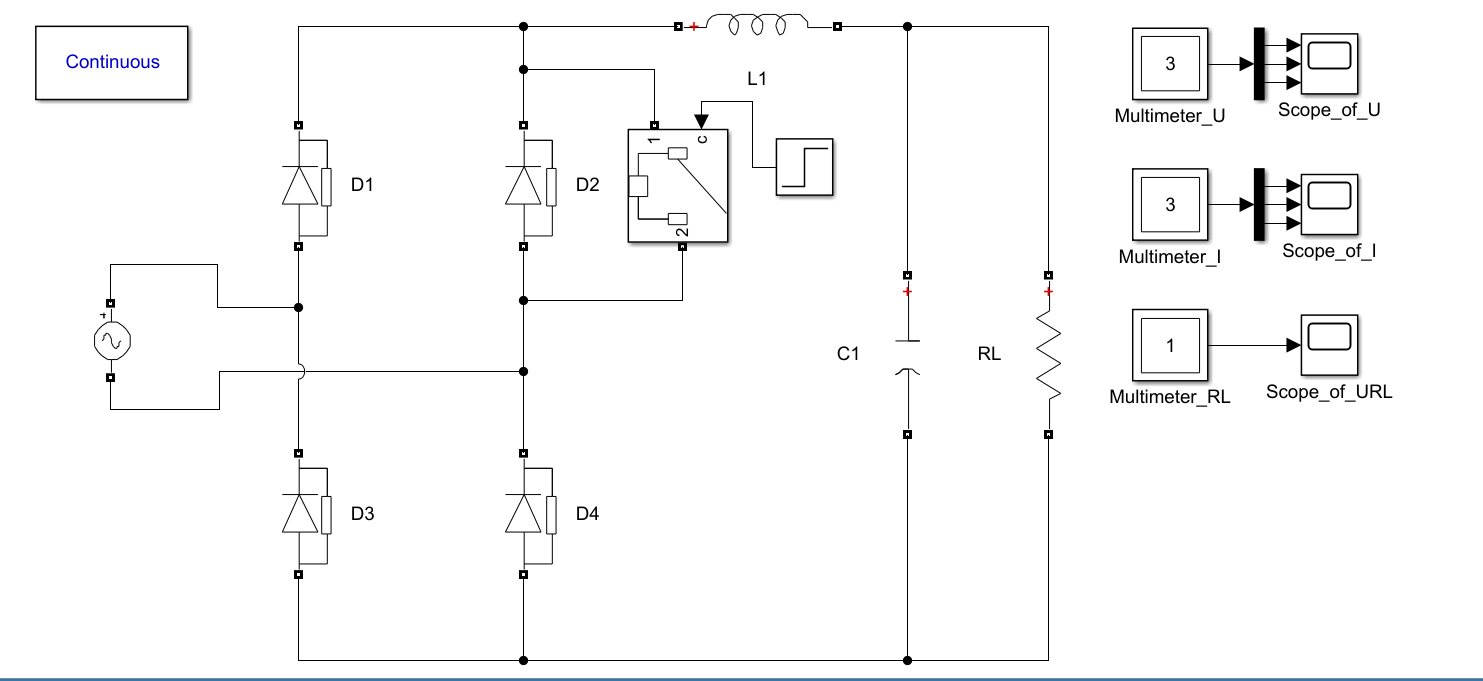
\includegraphics[width=9cm]{figure/D2_S.png}
		\quad
		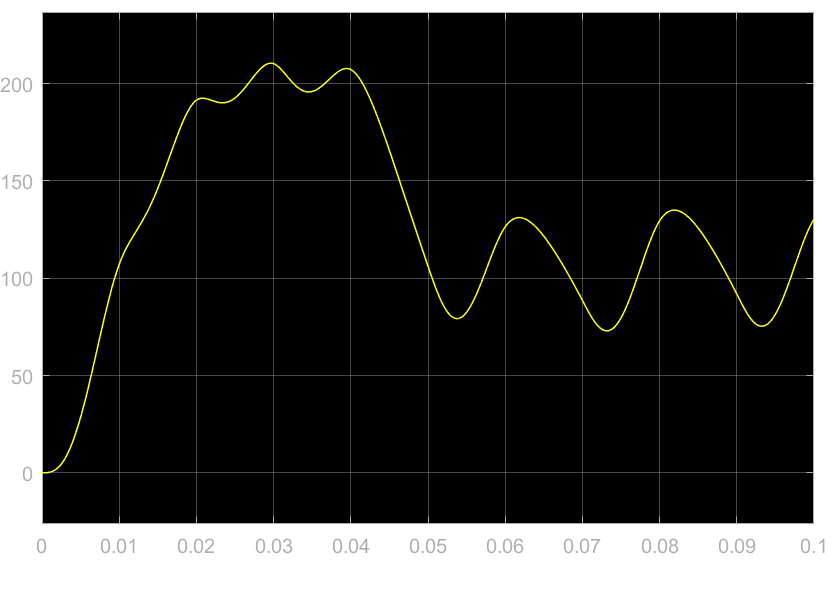
\includegraphics[width=5cm]{figure/D2_S_URL.png}
		\caption{二极管D2短路}
	\end{figure}
	
	\begin{figure}[bhtp]
		\centering
		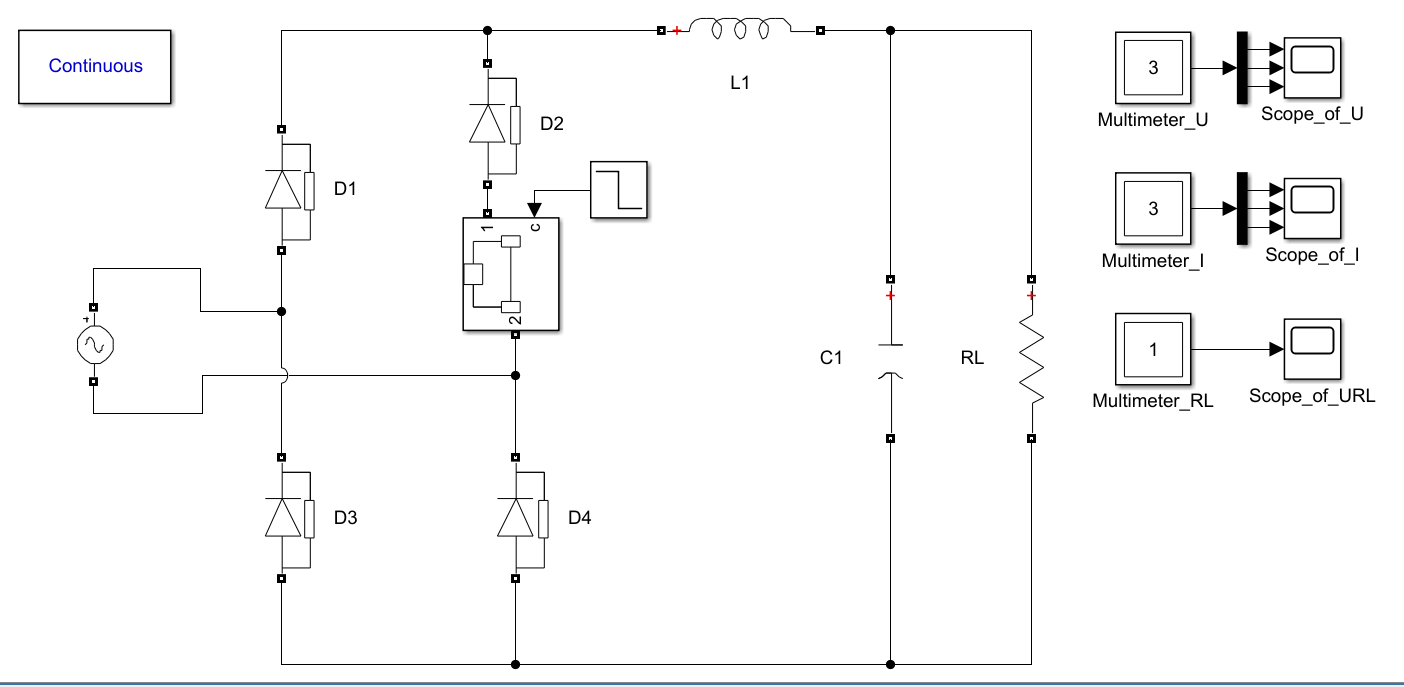
\includegraphics[width=9cm]{figure/D2_O.png}
		\quad
		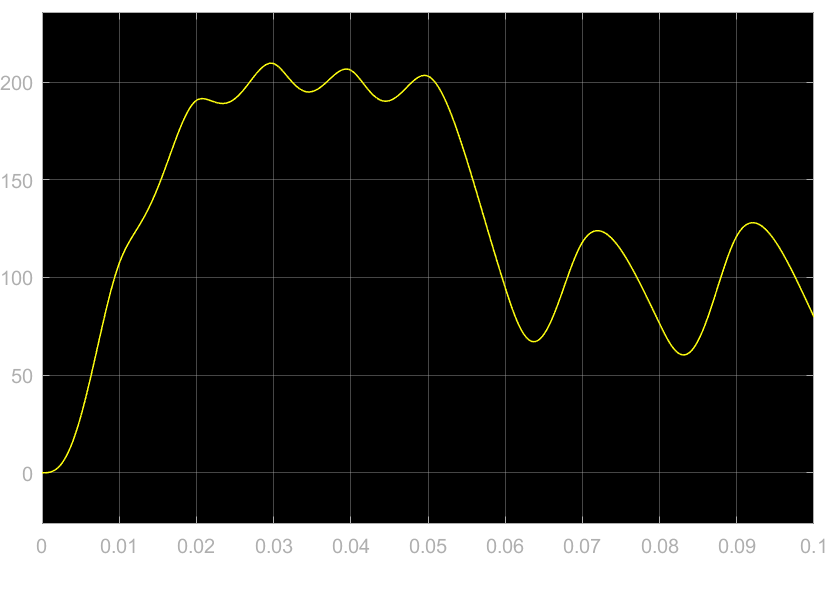
\includegraphics[width=5cm]{figure/D2_O_URL.png}
		\caption{二极管D2开路}
	\end{figure}
	
	\begin{figure}[bhtp]
		\centering
		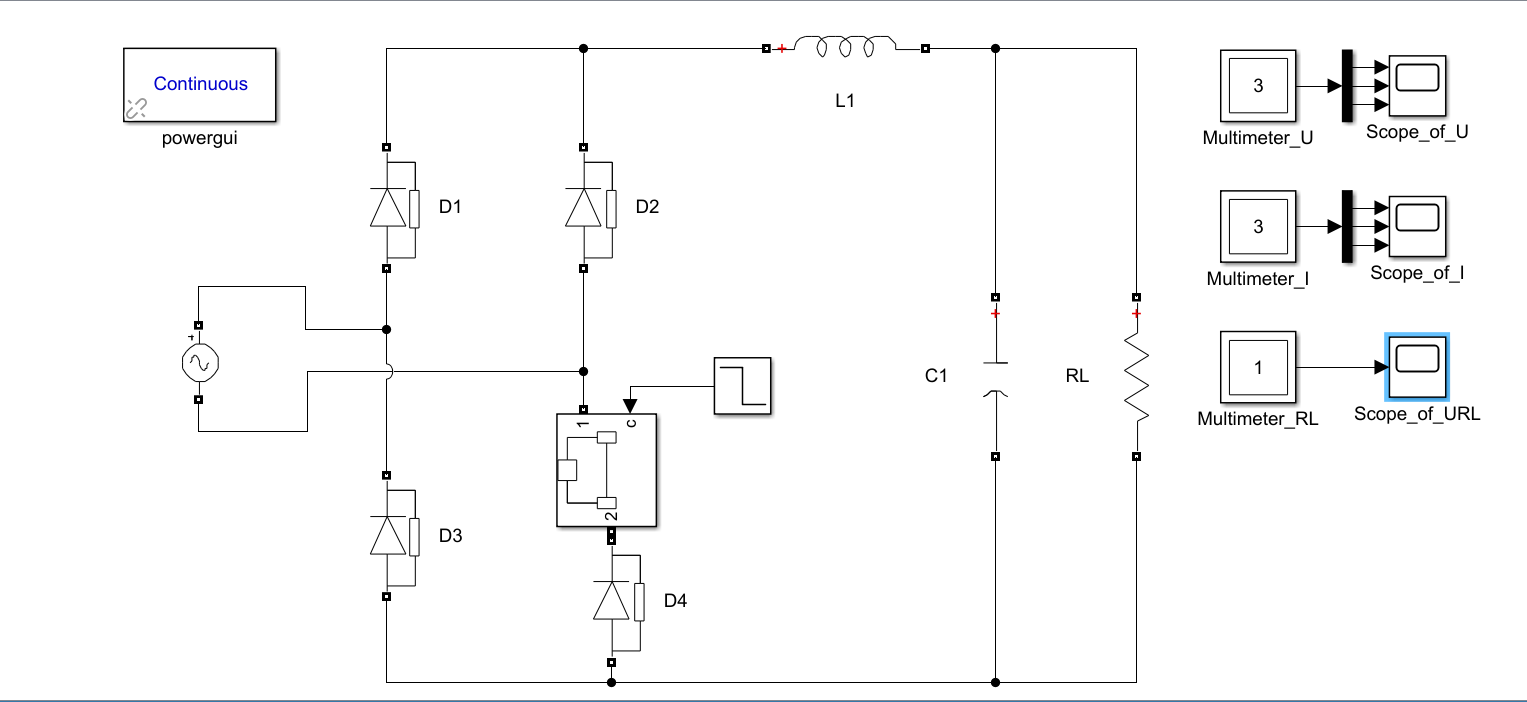
\includegraphics[width=9cm]{figure/D4_O.png}
		\quad
		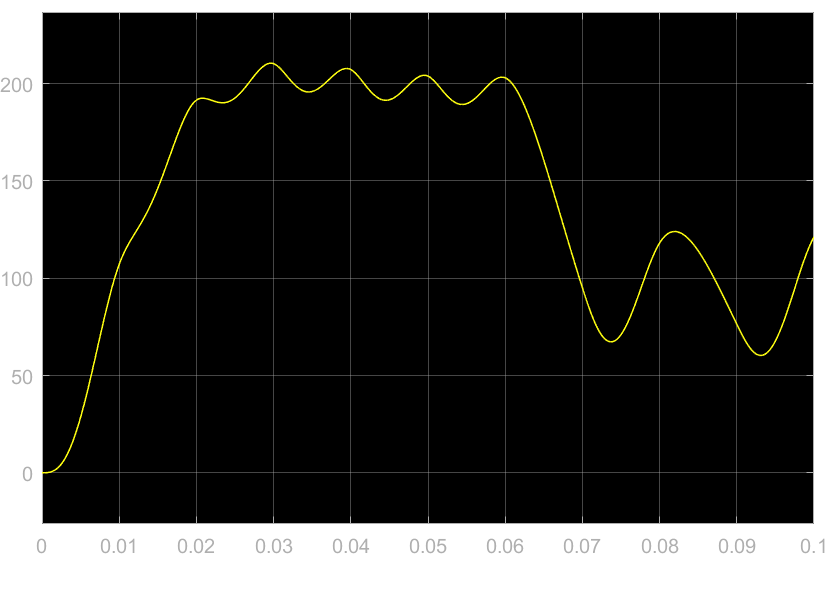
\includegraphics[width=5cm]{figure/D4_S_URL.png}
		\caption{二极管D4开路}
	\end{figure}
	
	\begin{figure}[bhtp]
		\centering
		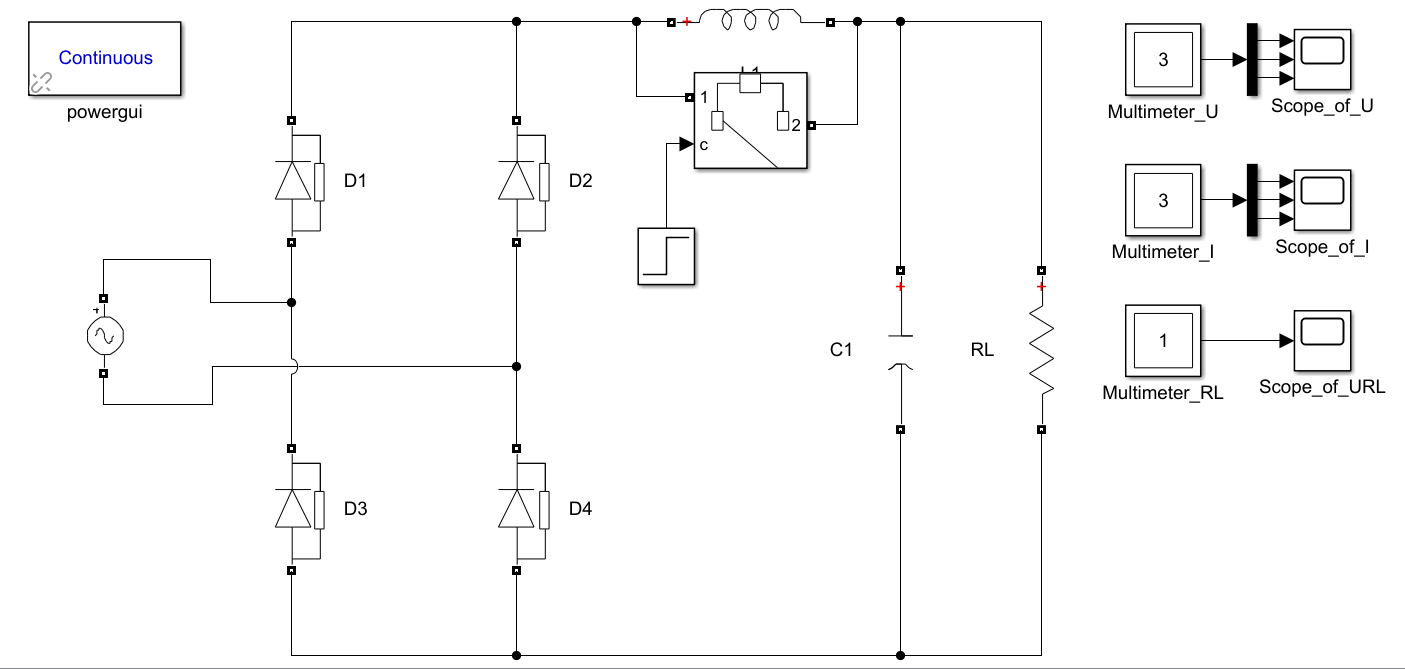
\includegraphics[width=9cm]{figure/L_O.png}
		\quad
		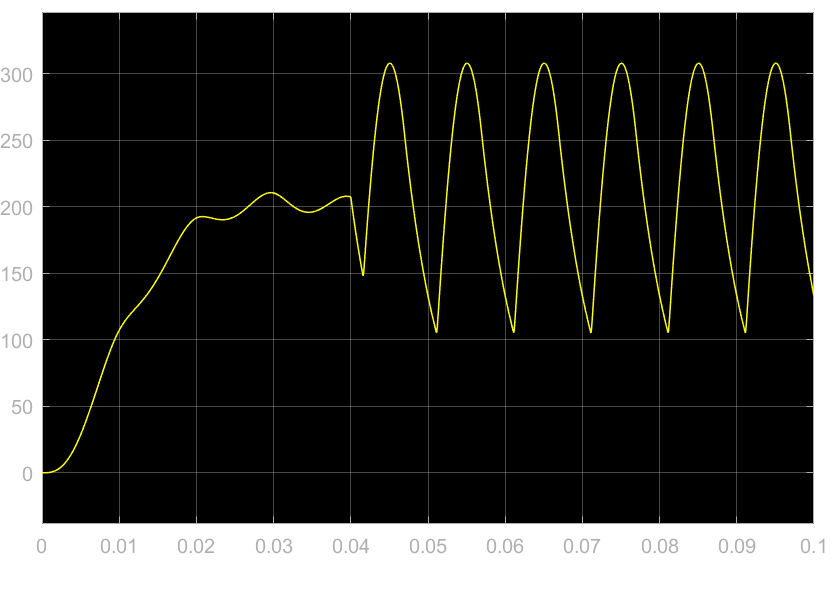
\includegraphics[width=5cm]{figure/L_O_URL.png}
		\caption{电感L开路}
	\end{figure}
	
	
	可以看出,不同电路故障在负载电压波形图上确实表现出了不同的特点。但是,原始数据太少,只有五张图。
	
	\section{对样本集的拓展处理}
	
	我首先采用了改变图像亮度的方式,将每一张原始图片按照亮度从原先的0.2倍变化到1.8倍。这样处理后图片数量达到了300张,虽然不是很多,但是先用来进行原理性实验。
	
	然后在后面设计网络的时候,我又采用了imageDataAugmente函数,在每一轮迭代开始前都将图片进行一个随机小比例的旋转和平移,这样就相当于有了总图片数$\times$迭代轮数张图片。
	
	在这里,我有一个疑问,就是对图像进行裁剪扩大数据集时,被裁减的部分该怎么处理,如果是将裁剪后的图片放大到原先的图片大小,波形的形状可能会受到拉伸这样的改变,如果是用0填充,又会不会产生影响?所以我没有对图像做裁剪处理,如果这个问题得到解决后,可以产生更多的样本数据集。
	
	另外,这一部分给我的感觉,就像是在做一个图像识别的问题,而与电路相关性不大。有没有一种可能性,是针对波形的相关处理,达到数据增强的效果,而不是对图片的处理。
	
	\section{基于Matlab的简单卷积神经网络搭建}
	
	这一部分我使用Matlab中的深度网络设计器APP进行网络设计,网络构造及具体参数见下图:
	
	\begin{figure}[htbp]
		\centering
		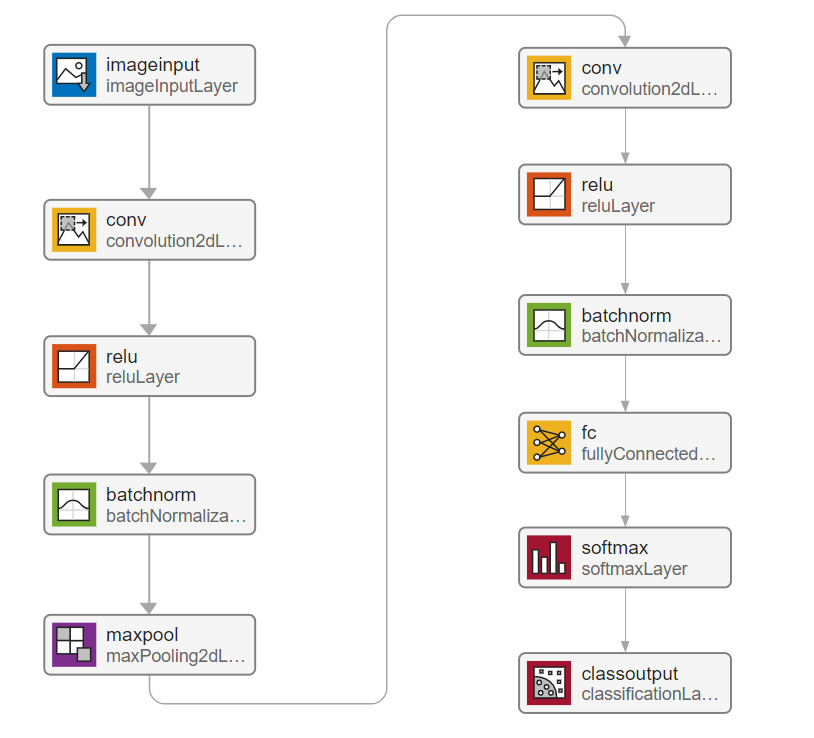
\includegraphics[width=6cm]{figure/net.png}
		\quad
		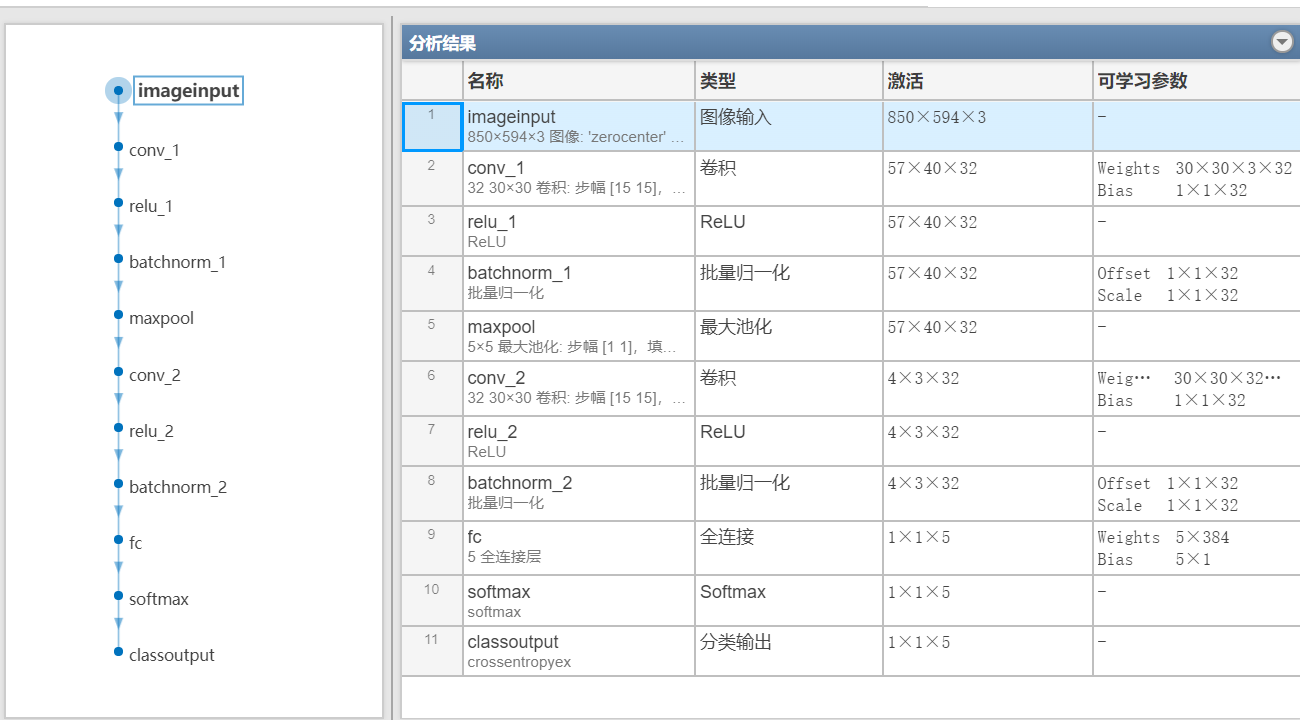
\includegraphics[width=10cm]{figure/net1.png}
		\caption{网络结构及具体参数}
	\end{figure}

	这个网络的结构是我从之前一次MNIST手写数据集识别中构建的网络改造过来的,我在原来的基础上去掉了一层卷积,简化了一下,然后对超参数的设定也凭感觉改了改。但是从后面训练的结果来看,发现分类不是很理想,所以这里我不清楚的就是,网络的结构和参数是否合理?这里能否从理论层面给出的选择依据和方法。
	
	模型代码如下:
	\begin{lstlisting}
	trainingSetup = load("D:\SRP_project\simple_examples" + ...
	"\params_2022_03_06__10_51_30.mat");
	
	imdsTrain = imageDatastore("D:\SRP_project\simple_examples\dataset",...
	"IncludeSubfolders",true,"LabelSource","foldernames");
	
	imageAugmenter = imageDataAugmenter(...
	"RandRotation",[0 20],...
	"RandScale",[1 10],...
	"RandXReflection",true,...
	"RandYReflection",true);
	
	augimdsTrain = augmentedImageDatastore([840 594 3],imdsTrain,...
	"DataAugmentation",imageAugmenter);
	
	opts = trainingOptions("sgdm",...
	"ExecutionEnvironment","auto",...
	"InitialLearnRate",0.01,...
	"Shuffle","every-epoch",...
	"Plots","training-progress",...
	"MiniBatchSize", 30);
	
	layers = [
	imageInputLayer([840 594 3],"Name","imageinput")
	
	convolution2dLayer([30 30],32,"Name","conv_1","Padding","same","Stride",[15 15])
	batchNormalizationLayer("Name","batchnorm_1")
	reluLayer("Name","relu_1")
	maxPooling2dLayer([5 5],"Name","maxpool_1","Padding","same")
	
	convolution2dLayer([30 30],32,"Name","conv_3","Padding","same","Stride",[15,15])
	batchNormalizationLayer("Name","batchnorm_3")
	reluLayer("Name","relu_3")
	
	fullyConnectedLayer(5,"Name","fc")
	softmaxLayer("Name","softmax")
	classificationLayer("Name","classoutput")
	];
	
	[net, traininfo] = trainNetwork(augimdsTrain,layers,opts);
	\end{lstlisting}
	
	\section{初步的训练尝试}
	
	按照前面的叙述,我进行了初步的训练,最终得到的结果并不是很满意,不断进行多次尝试调整参数后,最高的预测准确率只有76.67\%
	
	\begin{figure}[h]
		\centering
		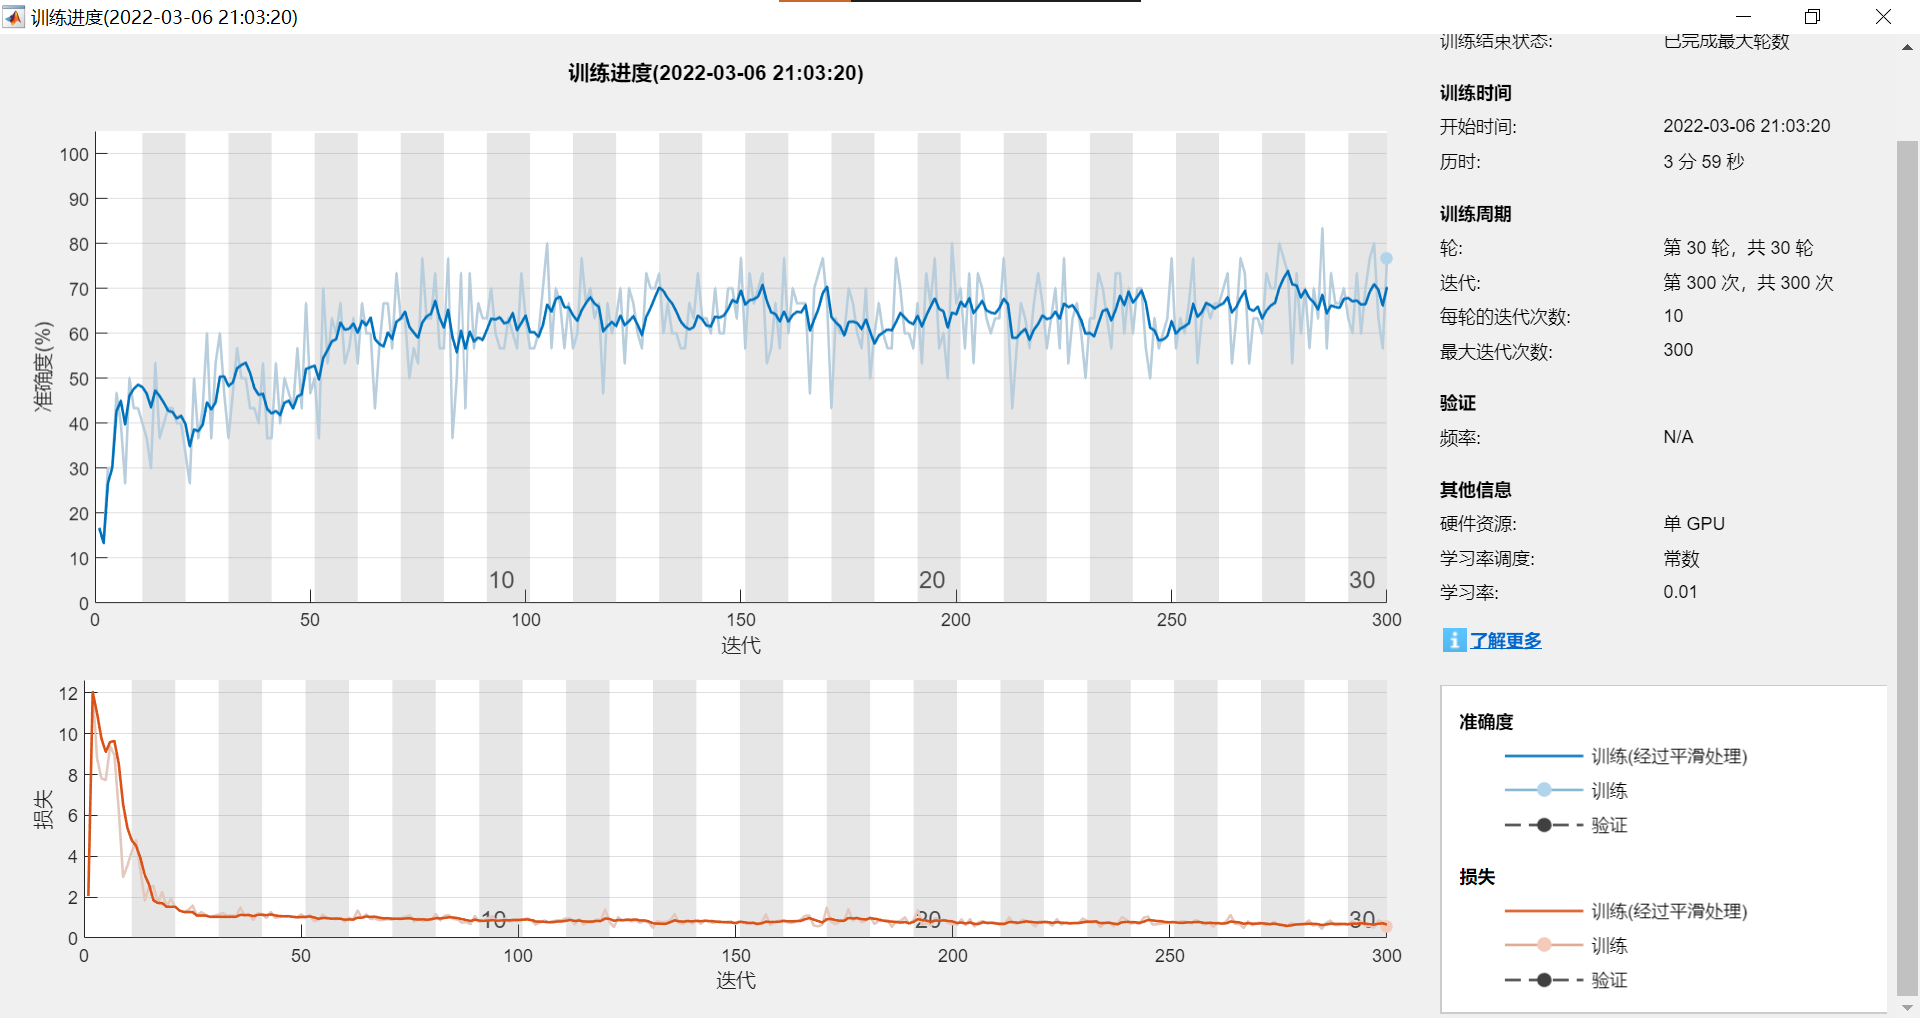
\includegraphics[width=15cm]{figure/第一次结果.png}
		\quad
		\includegraphics[width=15cm]{figure/第一次训练76.67\%.png}
		\caption{第一次训练}
	\end{figure}

	总而言之,这周先对整个流程进行了探索,打通了一些技术上的阻隔。如果方向问题不大的话,下一周探索一下怎样更好的解决样本数量少和训练精度不高的问题。
	
\end{document}